\documentclass{article}
\usepackage{tikz}
\usetikzlibrary{positioning}
\usetikzlibrary{shapes.geometric}
\usetikzlibrary{shapes.callouts}
\pagestyle{empty}

\begin{document}

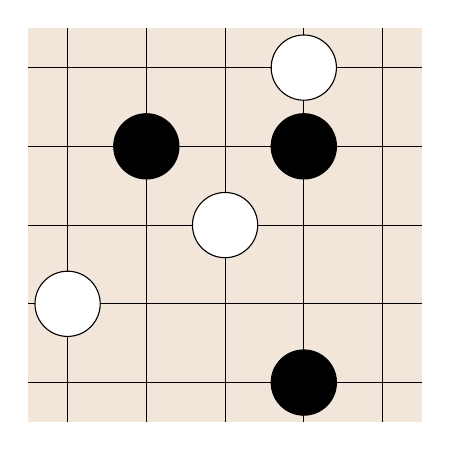
\begin{tikzpicture}
[stone/.style={shape=circle,draw=black,thin,scale=2.5},
  white/.style={stone,fill=white},
  black/.style={stone,fill=black}]

\draw [draw=none,fill=brown!20!white] (-2.5,-2.5) rectangle (2.5,2.5);
\draw[step=1] (-2.5,-2.5) grid (2.5,2.5);

\draw (-2,-1) node [white] {}
      (0,0) node [white] {}
      (1,2) node [white] {}
      (-1,1) node [black] {}
      (1,1) node [black] {}
      (1,-2) node [black] {};
\end{tikzpicture}
\end{document}
